\subsection{Fast API}\label{sec:API}
Die Fast API\autocite{FastAPI} ist eine der am häufigsten verwendeten Frameworks für die Entwicklung von Webanwendungen in der Programmiersprache Python. Frameworks sind Ansammlungen von Bibliotheken, Code und anderen Entwicklungstools, sie sollen die Entwicklung von Softwareanwendungen erleichtern. Eine Fast API kann ab einer Python Version von 3.6 erstellt werde. Die API ist eine Schnittstelle die es verschiedenen Anwendungen ermöglicht miteinander zu kommunizieren und Daten auszutauschen.\\
\vspace{3mm}
Das vorher erstellte Testprogramm wird umgeschrieben und zur API hinzugefügt. Später wird die API zu einem HTML Skript hinzugefügt. Durch das HTML Skript erhalten wir eine Webaplikation. Die API ist somit die Schnittstelle zwischen dem Python Code und dem HTML Skript.\\
\vspace{3mm}
\subsubsection{Erstellen einer Fast API}
Zuerst wird eine virtuelle Umgebung in VS-Code erstellt. Die Befehle werden alle im Terminal eingegeben.
\begin{verbatim}
python -m venv env
\end{verbatim}
Die virtuelle Umgebung mit dem Name \textit{env} wurde erstellt, jedoch ist diese noch nicht aktiviert. Mit dem unten angeführten Befehl wird die Umgebung aktiviert. 
\begin{verbatim}
source env/bin/activate
\end{verbatim}
Nachdem die virtuelle Umgebung aktiviert ist, kann die Fast API installiert werden. 
\begin{verbatim}
pip install fastapi
\end{verbatim}
Die API funktioniert nicht ohne lokalen Webserver. Hierfür eignet sich der Server Uvicorn. Uvicorn\autocite{uvicorn} ist ein schneller Webserver für Python Entwicklungen.  
\begin{verbatim}
pip install uvicorn
\end{verbatim}
Um den API-Server zu starten wird der folgende Befehl in das Terminal eingegeben.
\begin{verbatim}
uvicorn main:app --reload
\end{verbatim}
In VS-Code kann ein neues Programm erstellt werden. Wichtig ist das die Fast API eingebunden wird und eine Instanz festgelegt wird.
\begin{verbatim}
from fastapi import FastAPI
app = FastAPI()
\end{verbatim}

Es gibt verschiedene Dekoratoren die einer Funktion zugewiesen werden können. Ein Dekorator ist eine Funktion die einem bestimmten Teil eines Codes, eine Funktionalität zuweist. Mit dem Dekorator GET können Inhalte generiert und zurückgegeben werden. Durch den Dekorator POST, können verschieden Funktionen aufgerufen und Daten verarbeitet werden. GET und POST\autocite{GETvsPOST} sind die wichtigsten HTTP-Requests. Diese Requests können ganz einfach eingebunden werden:
\vspace{3mm}
\begin{figure}[H]
    \centering
    \begin{minted}{python}
                        app@get("/url")
                        app@post("/url")
    \end{minted}
    \caption{API-Dekoratoren}
\end{figure}
\begin{itemize}
    \item app, ist die vorher definierte Instanz
    \item @get, ist der Dekorator
    \item ("/URL"), URL wird angegeben.  
\end{itemize}

Als URL wird in diesem Fall nur ein Wort genommen. Mit der URL \textit{/docs} wird die Swagger UI\autocite{SwaggerUI} angezeigt. Auf der Swagger UI werden die vorher definierten GET- und POST-Requests dargestellt. \\

\begin{figure}[H]
    \centering
    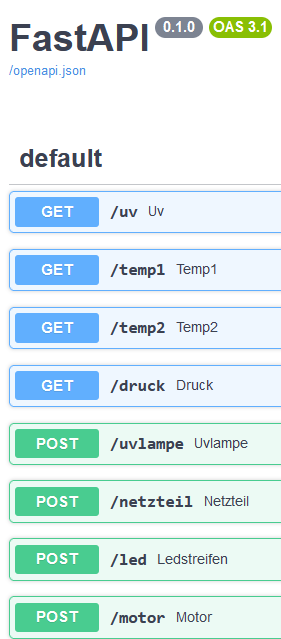
\includegraphics[scale=1.3]{image/fastapi.png}
    \caption{Beispiel Swagger UI}
    \label{fig:enter-label}
\end{figure}
\vspace{3mm}
Die Daten des Temperatursensors werden entweder in der Swagger UI ausgegeben oder unter der URL /temp1
\pagebreak
\subsubsection{Temperatursensor}\label{sec:API-Temp}
\begin{figure}[H]
    \centering
    \begin{minted}{python}
    @app.get("/temp1")
    def temp1():
        dhtDevice1 = adafruit_dht.DHT22(board.D7)
        temp_c = dhtDevice1.temperature
        humidity = dhtDevice1.humidity
        return{"Temperatur":temp_c , "Feuchtigkeit": humidity}
    \end{minted}
    \caption{API-Programm Temperatursensor}
\end{figure}
Damit der Code funktioniert muss die vorher heruntergeladene Bibliothek eingebunden werden. 
\begin{verbatim}
import adafruit_dht
\end{verbatim}
In der Funktion \textit{temp1} wird dem Sensor einen GPIO-Pin zugewiesen. Danach werden die Temperatur sowie die Feuchtigkeit durch eine vorgefertigte Funktion aus der Bibliothek abgefragt und ausgegeben.

\subsubsection{UV-Sensor}\label{API-UVS}
\begin{figure}[H]
    \centering
    \begin{minted}{python}
    @app.get("/uv")
    def uv():
        i2c = board.I2C()
        ltr = adafruit_ltr390.LTR390(i2c)

        while True:
            return("UV-Index:", ltr.uvi, 
                   "Umgebungslicht in Lux:", ltr.light)
            time.sleep(1.0)
    \end{minted}
    \caption{API-Programm UV-Sensor}
\end{figure}
\newpage

\subsubsection{Drucksensor}\label{sec:API-Druck}
Der Drucksensor gibt Daten über die I2C-Schnittstelle zurück. Diese Schnittstelle wird in der Funktion initialisiert. Damit die Messungen bzw. die Umrechnungen zu einem sinnvollen Ergebnis führen, muss der mittlere Luftdruck bei Meereshöhe angegeben werden. Dieser beträgt 1013.25 hPa. Der Druck und die Meereshöhe können durch Funktionsaufrufe abgefragt werden. 
\vspace{3mm}
\begin{figure}[H]
    \centering
    \begin{minted}{python}
    @app.get("/druck")
    def druck():
        i2c = board.I2C()
        bmp = bmp180.BMP180(i2c)
        bmp.sea_level_pressure = 1013.25
        return{f"Druck: {bmp.pressure:.1f} hPa", 
                f"Meereshöhe: {bmp.altitude:.1f} Meter"} 
    \end{minted}
    \caption{API-Programm Drucksensor}
\end{figure}

Um Bibliothek circuitpython-bmp180 verwenden zu können, muss diese im Programm eingebunden werden. Mit der unten angeführten Codezeile wird die Bibliothek zum Programm hinzugefügt. 
\begin{verbatim}
import bmp180
\end{verbatim}


\subsubsection{Schalten zwischen High und Low}\label{sec:Einschalten}
Es gibt einige Komponente, die eine ähnlichen Code besitzen. Diese wurden in diesem Kapitel zusammengefasst und anhand eines Beispiels erklärt. Für diesen Teil des Codes wird keine Bibliothek benötigt, es wird nur die Tasterabfrage aus dem Kapitel \ref{sec:Tasterabfrage} verwendet. Der unten stehende Code zieht einen Pin auf High oder auf Low. Das sorgt dafür das die Komponente ein- und ausgeschalten werden könne. Dieser Code giltet für folgende Komponente:
\begin{itemize}
    \item UV-Lampe
    \item Netzteil
    \item Kühlung
    \item Lüftung
\end{itemize}
Der Code wird anhand der UV-Lampe erklärt. Wenn der Code ausgeführt wird, wird in der Swagger UI etwas zurückgegeben. Entweder UV-Lampe eingeschaltet und UV-Lampe ausgeschaltet.\\
\vspace{3mm}
\begin{figure}[H]
    \centering
    \begin{minted}{python}
    @app.post("/uvlampe")
    def uvlampe():
        global boolUV
        boolUV = not boolUV
        if boolUV == True :
            GPIO.output(PinUV,GPIO.HIGH)
            return{"UV-Lampe eingeschaltet"}
        else:
            GPIO.output(PinUV,GPIO.LOW)
            return{"UV-Lampe ausgeschaltet"}
    \end{minted}
    \caption{API-Programm UV-Lampe}
\end{figure}
Der Code kann ganz einfach auf andere Komponente umgeschrieben werde. Die Variablen müssen nur umbenannt werden und der gewünschte Satz der ausgegeben werden soll, abgeändert werden.
\vspace{3mm}
\begin{figure}[htbp]
    \centering
    \begin{subfigure}[b]{0.4\textwidth}
        \centering
        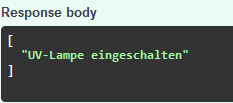
\includegraphics[width=\textwidth]{image/uvlampe ein.png}
        \caption{UV-Lampe eingeschaltet}
        \label{fig:bild1}
    \end{subfigure}
    \hfill
    \begin{subfigure}[b]{0.35\textwidth}
        \centering
        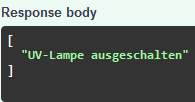
\includegraphics[width=\textwidth]{image/UVLampe aus.png}
        \caption{UV-Lampe ausgeschaltet}
        \label{fig:bild2}
    \end{subfigure}
    \caption{API-Ausgabe UV-Lampe}
    \label{fig:zwei_bilder}
\end{figure}


\subsubsection{Motor und Endschalter}
Das Programm sieht genau gleich aus wie im Testprogramm (Kapitel \ref{sec:test motor}). Zu beachten ist, dass ein Thread verwendet werden muss. Da die API den Code nur einmal ausführt. Wird jedoch ein Thread verwendet, bearbeitet er die "in range" Schleife. 
